%%
%% Copyright 2022 OXFORD UNIVERSITY PRESS
%%
%% This file is part of the 'oup-authoring-template Bundle'.
%% ---------------------------------------------
%%
%% It may be distributed under the conditions of the LaTeX Project Public
%% License, either version 1.2 of this license or (at your option) any
%% later version.  The latest version of this license is in
%%    http://www.latex-project.org/lppl.txt
%% and version 1.2 or later is part of all distributions of LaTeX
%% version 1999/12/01 or later.
%%
%% The list of all files belonging to the 'oup-authoring-template Bundle' is
%% given in the file `manifest.txt'.
%%
%% Template article for OXFORD UNIVERSITY PRESS's document class `oup-authoring-template'
%% with bibliographic references
%%

%%%CONTEMPORARY%%%
%\documentclass[unnumsec,webpdf,contemporary,large]{oup-authoring-template}%
%\documentclass[unnumsec,webpdf,contemporary,large,namedate]{oup-authoring-template}% uncomment this line for author year citations and comment the above
%\documentclass[unnumsec,webpdf,contemporary,medium]{oup-authoring-template}
%\documentclass[unnumsec,webpdf,contemporary,small]{oup-authoring-template}

%%%MODERN%%%
\documentclass[unnumsec,webpdf,modern,large]{oup-authoring-template}
%\documentclass[unnumsec,webpdf,modern,large,namedate]{oup-authoring-template}% uncomment this line for author year citations and comment the above
%\documentclass[unnumsec,webpdf,modern,medium]{oup-authoring-template}
%\documentclass[unnumsec,webpdf,modern,small]{oup-authoring-template}

%%%TRADITIONAL%%%
%\documentclass[unnumsec,webpdf,traditional,large]{oup-authoring-template}
%\documentclass[unnumsec,webpdf,traditional,large,namedate]{oup-authoring-template}% uncomment this line for author year citations and comment the above
%\documentclass[unnumsec,namedate,webpdf,traditional,medium]{oup-authoring-template}
%\documentclass[namedate,webpdf,traditional,small]{oup-authoring-template}

%\onecolumn % for one column layouts

%\usepackage{showframe}

\graphicspath{{Fig/}}

% line numbers
%\usepackage[mathlines, switch]{lineno}
%\usepackage[right]{lineno}

\theoremstyle{thmstyleone}%
\newtheorem{theorem}{Theorem}%  meant for continuous numbers
%%\newtheorem{theorem}{Theorem}[section]% meant for sectionwise numbers
%% optional argument [theorem] produces theorem numbering sequence instead of independent numbers for Proposition
\newtheorem{proposition}[theorem]{Proposition}%
%%\newtheorem{proposition}{Proposition}% to get separate numbers for theorem and proposition etc.
\theoremstyle{thmstyletwo}%
\newtheorem{example}{Example}%
\newtheorem{remark}{Remark}%
\theoremstyle{thmstylethree}%
\newtheorem{definition}{Definition}
\usepackage{parskip}
\usepackage{amsmath}
\usepackage{graphicx}
\usepackage[numbers]{natbib}
\usepackage{float}

\begin{document}

\journaltitle{Bioinformatics}
\DOI{DOI HERE}
\copyrightyear{2024}
\pubyear{2024}
\access{Advance Access Publication Date: Day Month 2024}
\appnotes{Original Paper}

\firstpage{1}

\subtitle{Structural bioinformatics}

\title{Robustness of Deep Learning with Graph Convolutional Networks in Multi-Omics Data Integration for Small Clinical Samples}

\author{Giuliana Orizzonte\ORCID{0000-0000-0000-0000}}
\author{Hae-Won Uh}
\author{Said el Bouhaddani}

\authormark{Orizzonte et al.}

\address{\orgdiv{Julius Center, dept. Data Science and Biostatistics}, \orgname{University Medical Center Utrecht}, \orgaddress{\street{Universiteitsweg 100}, \postcode{3584 CG}, \country{Utrecht, The Netherlands}}}

\corresp[$\ast$]{Corresponding author. \href{email:email-id.nl}{g.orizzonte@uu.nl}}

\received{Date}{0}{Year}
\revised{Date}{0}{Year}
\accepted{Date}{0}{Year}

\abstract{
\textbf{Motivation:} .\\
\textbf{Results:} .\\
\textbf{Availability and Implementation:} .\\
\textbf{Supplementary information:} The softare is available at https://github.com/gorizzonte}

\maketitle

\section{Introduction}
Recent advancements in the life sciences resulted in an unprecedented abundance of biological data. The data, although comprehensive, is often characterized by small sample sizes, high dimensionality, and heterogeneous measurement techniques \cite{misra2019integrated}. Even a single cell exhibits a myriad of molecular interactions and pathways, spanning layers of biological functions that include genomics, transcriptomics, proteomics, metabolomics, and more, all of which constantly interact \cite{aranda2010intact, cordell2009detecting}. These diverse layers of molecular information are collectively referred to as multi-omics \cite{vailati2017omics}. Each omics layer produces data of varying scales, formats, and dimensions, and the process of combining information is known as multi-omics data integration \cite{athieniti2022guide, Bouhaddani2023, subramanian2020multi}. Multi-omics integration can help understand disease mechanisms, treatment responses, and individual variations at a molecular level \cite{dihazi2018integrative}. By integrating genomics, transcriptomics, proteomics, metabolomics, etc. researchers can analyze the biological processes involved in diseases as a whole \cite{Hasin2017, duan2021evaluation}. For instance, by analyzing gene expression (transcriptomics) alongside protein activity (proteomics), scientists can trace how genetic alterations influence protein function and cellular behavior \cite{guil2015rna}. This approach can identify biomarkers for diagnosis, prognosis, and therapy development \cite{hann2001molecular, karczewski2018integrative, mendez2017many}.

\par However, traditional analytical techniques have limitations that hinder such a global analysis; often they are limited to single omics analyses or restrict relations between omics to be linear \cite{Wu2021, stahlschmidt2022multimodal, singh2019diablo}. Additionally, they overlook complex, non-linear interactions, which could render the results incomplete \cite{picard2021integration, reel2021using, tolani2021big}. Deep-learning methods, particularly Neural Networks (NNs), have furthered multi-omics data analysis because they excel in identifying patterns and inferring relationships from large, multi-dimensional datasets \cite{wen2023deep, Brombacher2022, leng2022benchmark}. For instance, they can recognize patterns in gene expression data that may be indicative of disease states or therapy responses \cite{tong2020deep, huang2019salmon, nicora2020integrated}. Graph Neural Networks (GNNs) are a class of NN models that deal with graph-structured data \cite{cui2022graph}. The graph structure can reproduce existing biological networks, such as protein-protein interaction networks or gene regulatory networks \cite{Milano2023}. This structural similarity enables GNNs to simultaneously capture biological entities (e.g., proteins, genes) as well as their interactions \cite{Zhu2023, Wang2020, wang2020moronet}. In such graphs, entities are represented as nodes while connections between nodes are represented as edges. GNNs also allow for message-passing algorithms, whereby nodes send and receive 'messages', i.e., information, to and from their neighbors \cite{Li2022Pan, tang2022graph}. The shared information is used to update the features of each node. 

\begin{figure*}[!t]%
\centering
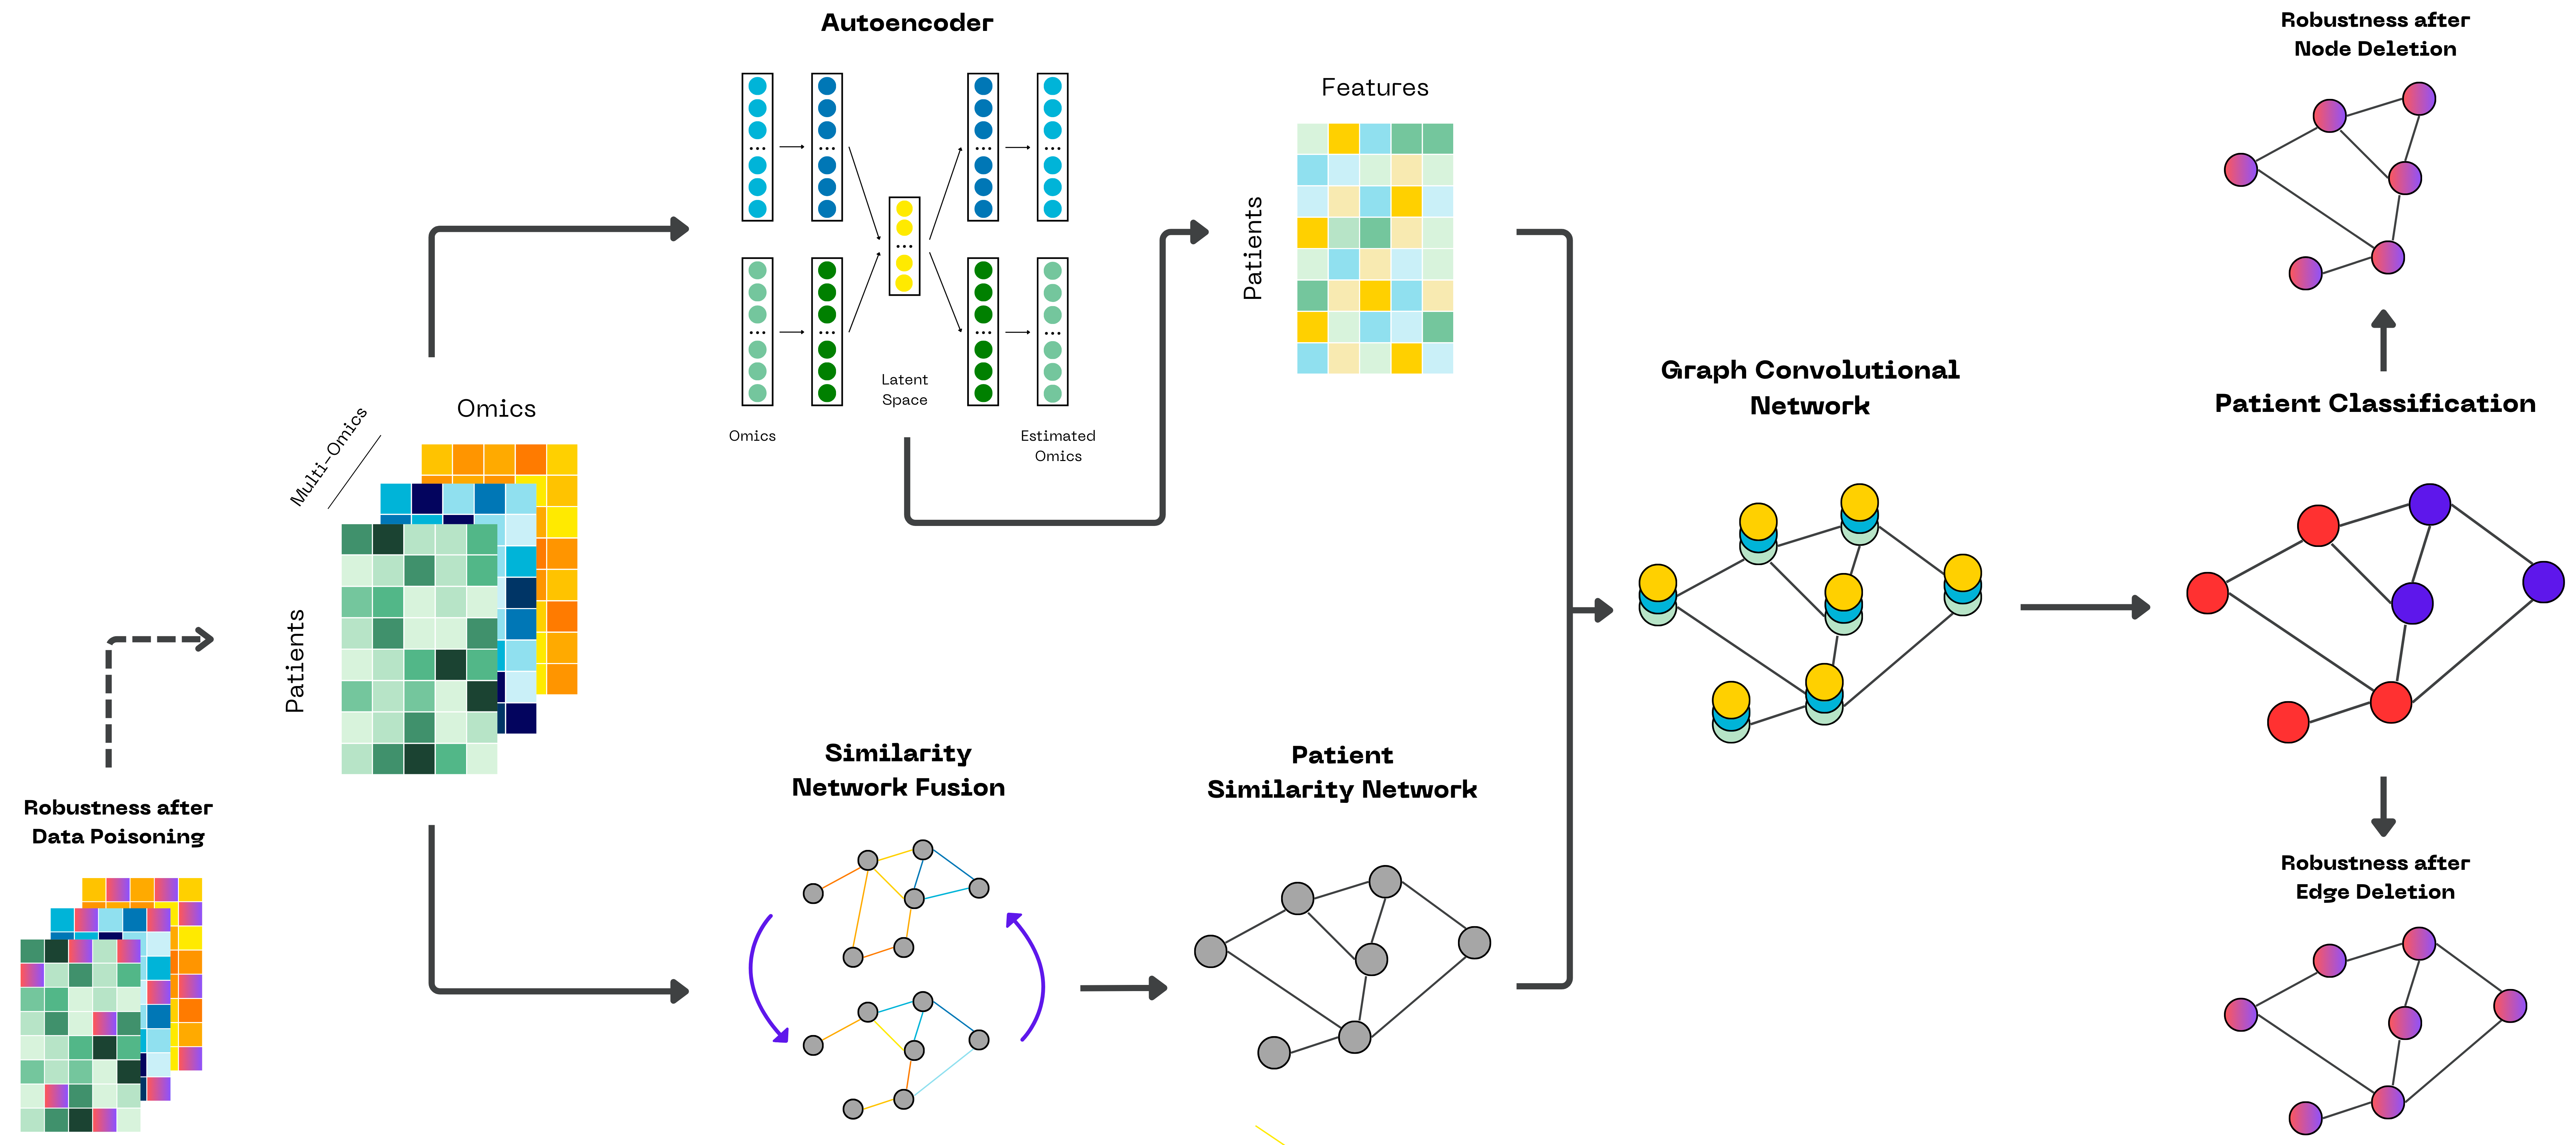
\includegraphics[width=\textwidth]{Robustness after Data Poisoning(1).png}
\caption{Schematic of the model's workflow. The multi-omics datasets are the initial input. The Autoencoder is used to capture meaningful variation across omics while creating a matrix of lower dimensions that is used as a features matrix by the GCN. The SNF is used to construct a PSN that captures similarity in omics variation between patients. This pattern of connections forms the input adjacency matrix to the GCN. The features matrix and adjacency matrix are fed into the GCN, which is trained to perform node (i.e., patient) classification. The Autoencoder to Patient Classification analyses are part of the MoGCN framework. Finally, three adversarial attacks involving node deletion, edge deletion, and data poisoning are used to test its Robustness.}\label{fig2}
\end{figure*}

The iterative process allows GNNs to refine the representation of each node based on its local neighborhood, capturing both individual characteristics and the broader context of its connections \cite{Wu2022, Zhang2023}. This mechanism is useful in the analysis of biological systems because the functions and behaviors of an entity are determined by both its properties and its interactions \cite{Althubaiti2021, Song2021, Wang2021}. For instance, in a gene regulatory network, the activity of a gene is influenced by its regulatory elements and the interacting proteins. Graph Convolutional Networks (GCNs) are a subset of GNNs that aggregate information through convolutions \cite{kipf2016semi, tang2022graph}. Convolutions involve a linear aggregation of features from neighbors, followed by a weighted transformation and a nonlinear activation function. GCNs offer the advantages of simplicity and efficiency, and have been successfully implemented in multi-omics integration \cite{Liu2020, Li2021, Gao2023, Schulte2021}. 

Nevertheless, deep-learning models including GCNs also have disadvantages. A key challenge is the limited availability of large datasets, particularly for randomized controlled trials (RCTs). Small samples can lead to overfitting, a situation where models perform well on training data but fail to generalize to new data \cite{Wu2022}. It is not known how the performance of GNNs in multi-omics integration may be affected by a small sample size, given that previous research uses data from large databases \cite{Althubaiti2021, Liu2020, Li2021, Li2022}. Additionally, deep learning models are highly sensitive to input variations, meaning that small changes can lead to different predictions \cite{zugner2020adversarial}. This can be an issue for robustness, i.e., a model’s ability to perform at a similar capacity when provided with noisy data. One of the techniques used to estimate the robustness of deep-learning models is Adversarial Robustness \cite{Günnemann2022}. Adversarial robustness involves intentionally introducing small perturbations to the input data, known as “attacks”, to test the model's resilience. A robust model can learn meaningful representations from the data, whereas a model that is not robust cannot distinguish meaningful patterns from noise \cite{eykholt2018robust}. Knowing when or why a model fails an adversarial attack can inform the development of an alternative model.

I consider a deep learning model that includes a GCN on multi-omics data obtained from an RCT and subsequently perform tests of Adversarial Robustness with two specific goals: (1) evaluate the performance of GCNs with small clinical samples and compare that with the performance of GCNs on large database samples found in the literature; (2) investigate the robustness of GCNs to assess changes in performance when presented with perturbed multi-omics data. 
To achieve these goals, I utilize multi-omics data from participants in the TOFA-predict study, an RCT study conducted to assess the efficacy of tofacitinib, a medication for the treatment of Psoriatic Arthritis (PsA) \cite{kleinrensink2022tofa}. PsA is a heterogeneous inflammatory disease whose pathobiology is poorly understood; thus, omics data are tools used to explore its underlying biological processes \cite{kleinrensink2022tofa}. The study includes two patient groups: newly diagnosed patients, dubbed naïve, and previously diagnosed patients who received pharmacological treatment but did not respond to it, dubbed resistant. In the 4-arm RCT half of each group is randomly assigned to Tofacitinib or alternative treatment and there are multiple follow-up moments. However, I focus exclusively on the multi-omics data that was collected at baseline. The primary objective of this research is to test whether the resistant patients exhibit distinct data patterns. If the resistant patients can be successfully identified using multi-omics data, medical professionals could use insights from the model’s interpretation to identify potential biomarkers for response to pharmacotherapy and to understand the molecular mechanisms of RA and its progression.

\section{Methods}

I consider the MoGCN framework for data analysis and prediction \cite{Li2022}. MoGCN is a deep learning model that utilizes multi-omics data for node classification, where a node may represent a patient or a sample. It consists of multiple components: an Autoencoder, a Similarity Network Fusion, and a GCN. Following the prediction task, the robustness of the model against adversarial attacks is investigated. The analyses are performed in Python with Pandas, Pytorch, and Snfpy.

\subsection{Data}

The omics data were measured from plasma samples and included one proteomics profile and four metabolomics profiles. The proteomics data were measured with Olink Proteomics technology, yielding 368 proteins. The metabolomics profiles were measured with UPLC-MS on four platforms: Amino acids, Signaling Lipids, Lipids, and Global. In the Amines profile, 57 compounds were identified using Study Quality Control (SQC) correction. For the Signaling Lipids profiling at high pH, 70 compounds were reported using SQC correction. For the Signaling Lipids profiling at low pH, 92 compounds were identified using SQC correction. Currently, the data for the Lipids and Global Metabolomics is still being processed.

\subsection{Autoencoder}

An autoencoder is a NN architecture used for unsupervised learning \cite{kingma2013auto, bohm2020probabilistic}. It's designed to compress the input data into a lower-dimensional representation and then reconstruct it back to the original form. It consists of two components: an encoder $f$ and a decoder $g$, which function in tandem. The encoder transforms data from its original domain to a compressed representation in a latent space $Z$ with lower dimensions $L$. Subsequently, the decoder reconstructs the data back into the original space from this latent space, thus $z = f(x)$ and $\tilde{x} = g(z)$. This architecture is designed to identify and retain critical features of the data by minimizing a reconstruction loss, which is a measure of how well the output of the autoencoder resembles the original input. For multi-omics, an autoencoder can reduce the dimensionality of the data, extracting the most relevant features while minimizing information loss and reducing noise.

\par In MoGCN \cite{Li2022}, the autoencoder is used to “condense” the multi-omics data from a three-dimensional structure (i.e., ${\text{gene} \times \text{patients} \times \text{omics}} $) into a two-dimensional matrix, which is later needed in the GCN. Thus, even though both the encoder and decoder are optimized, the focus is on the latent representations generated by the encoder, which reduce the multi-omics dimensions. The input data comprise five types of omics data, which are represented by the matrices $X_1,\ldots,X_5$. Because there is more than one input matrix, MoGCN utilizes a multi-modal autoencoder architecture. This structure consists of several encoders and decoders, each corresponding to an omic type, but all converging to a shared latent layer. The loss function in this multi-modal setup is an aggregate of weighted losses for each data type:
\begin{multline}
E = argmin_{f,g} (\alpha Loss_1 (x_1, g_1(f_1(x_1))) + \ldots \ + \\
\varepsilon Loss_5 (x_5, g_5(f_5(x_5))),\label{AE} 
\end{multline}
where $\alpha ,\ldots, \varepsilon$ are weights that reflect the relative importance or prior knowledge of each omics type, and they sum up to 1. This weighted approach can accommodate the nuances of each omics type.


\subsection{Similarity Network Fusion and Patient Similarity Network}

The Similarity Network Fusion (SNF) algorithm is designed to integrate different types of data by creating a network or graph where each node represents a sample and edges represent similarities between these samples \cite{wang2014similarity}. The SNF can be used to compute and combine Patient Similarity Networks (PSNs). First, the SNF calculates within-patient similarity matrices across omics. For $n$ patients the results are $n$ similarity matrices across omics. Then, these matrices are fused to construct a network that maps the similarities between patients. This process involves amplifying the strong connections and diminishing the weaker ones. The outcome of the fusion is one PSN that captures patterns across omics and patients. 

In MoGCN \cite{Li2022}, the fused PSN is what defines the structure of the graph for the GCN. Each patient is represented as a node and edges placed between patients represent similar omics patterns, effectively creating a network that mirrors the biological similarities between patients. With one patient $i$ and two omics $m, n$, the equation of the scaled exponential patient similarity matrix is:
\begin{equation}
    W(i, i) = \exp\left( -\frac{\rho^2(x_m , x_n)}{\mu \epsilon_{m, n}} \right),\label{PSN}
\end{equation}
where the ${\text{n} \times \text{n}}$ patient-patient similarity matrix is $W(i, j)$, $\rho(x_m, x_n)$ is the Euclidean distance between the patients' omics $x_m$ and $x_n$, $\mu$ is a hyperparameter that can be empirically set, and $\epsilon_{m, n}$ is a hyperparameter used to solve the problem of scaling. Different omics datasets have largely different scales, so when calculating the Euclidean distance it’s important to include a correction to prevent the larger scales from disproportionately influencing the distance calculation.

\par Then, the similarity matrix of two patients $P$ and K-nearest similarity matrix $S$ can be defined as
\begin{equation}
    P(i, j) = \begin{cases} 
    \frac{W(i, j)}{2\sum_{k \neq i} W(i,k)} & \mbox{if }j \neq i \\ 
    \frac{1}{2} & \mbox{otherwise},
    \end{cases}\label{SNF}
\end{equation}

\begin{equation}
    S(i, j) = \begin{cases} 
    \frac{W(i, j)}{\sum_{k \in N_i} W(i,k)} & \mbox{if }j \in N_i, \\ 
    0 & \mbox{otherwise}.
    \end{cases}\label{KSNF}
\end{equation}

When dealing with similarity matrices for multi-omics data, the matrices can be quite dense, with non-zero values indicating some level of similarity between all pairs of patients. However, these similarities are not all equally relevant, as a patient is more likely to be closely related to a small subset of other patients rather than all patients. The K-nearest similarity matrix is a version of the original matrix where for each patient only the similarities with their K-nearest neighbors are retained, and other connections are set to zero. This makes the matrix sparser and more focused. The similarity matrices can be iteratively updated to account for all patients. For the formulas describing this iterative process and the generalization to $m$ omics, readers can refer to the original MoGCN paper.

\subsection{Graph Convolutional Network}

The core concept of GNN architectures revolves around the iterative updating of node representations by integrating the representations of adjacent nodes with their own. At each layer of the GNN, information from the neighbors of each node is merged with an $AGGREGATE$ function and subsequently integrated with a $COMBINE$ function \cite{tang2022graph}. With $k$ layers, $\nu = {1, ..., n}$ nodes, and $N(\nu)$ denoting the neighbors of a node, the graph state H is defined as:
\begin{align*}
& \text{Initialization: } H^0 = X \\
& \text{For } k = 1, 2, \ldots, K, \\
& \quad \quad a_{\nu}^{k} = \textbf{AGGREGATE}^k\{H_{u}^{k-1} : u \in N(\nu)\} \\
& \quad \quad \quad \quad H_{\nu}^{k} = \textbf{COMBINE}^k\{H_{\nu}^{k-1}, a_{\nu}^{k}\}.
\end{align*}

After each layer, the combined representations become the new node representations. After the final layer, node representations are used for downstream tasks, for example node classification. The predicted label of a node $\hat{y_i}$ can be computed with a Softmax function. Training a GNN model involves minimizing a loss function, like cross-entropy. The network is optimized using backpropagation to minimize the objective function, in this case the discrepancy between predicted and observed node labels. GCNs are a subset of GNNs where the node representations in each layer are updated according to a propagation rule designed to approximate convolutional filters, which helps in linearizing the graph structure for computation \cite{kipf2016semi}.

\par In MoGCN \cite{Li2022}, the nodes of the GCN each represent one patient, while the edges between them represent similarity between patients as calculated with the PSN. The node features are the output of the Autoencoder, meaning that each patient is described using the latent representation of their multi-omics data. At each GCN layer, each patient's features are updated as such: (1) the latent representation of their omics data is aggregated with those of similar patients, and (2) the aggregated representations go through a convolution, creating a single new feature representation. At the final layer, each patient is assigned a label to classify them as naïve or resistant.

To assign patients labels, the GCN algorithm requires a graph structure and node features \cite{kipf2016semi}. The node features are contained in the feature matrix $X$, whose dimensions are $n$ (the number of nodes, i.e., patients), and $f$ (the number of features per node). The graph structure, i.e., its connections, are defined by adjacency matrix $A$. The GCN is constructed with multiple convolutional layers, each defined by the equation

\begin{equation}
    H^{k+1} = \sigma\left(\tilde{D}^{-\frac{1}{2}} \tilde{A} \tilde{D}^{-\frac{1}{2}} H^k W^k\right),
\end{equation}

where $\tilde{A} = A + I$ is the adjacency matrix $A$ plus self-connections $I$; $\tilde{D}$ is a diagonal matrix with $\tilde{D}_{ii} = \sum_j\tilde{A}_{ij}$; $\sigma(\cdot)$ is an activation function like ReLU; $H^k$ is the graph state; and $W^k$ is a linear transformation matrix to be trained \cite{tang2022graph}.

\subsection{Adversarial Robustness}

\par Investigating GCN robustness involves creating worst-case perturbations, i.e., minor data changes that lead to substantial output differences \cite{zugner2018adversarial}. Adversarial robustness can be framed as an optimization problem in which the goal is to find data perturbations that maximize certain attack objectives, such as promoting an incorrect classification \cite{Günnemann2022}. Adversarial attacks can vary depending on their scenario, type, and perturbation space \cite{Günnemann2022}. 

\par There are two scenarios: poisoning and evasion. With poisoning, perturbations occur before the model's training, impacting both the learning process and the resulting model. Evasion involves altering data during the testing phase, with the model already trained and fixed. Attack types can be local or global. Local attacks focus on how predictions for a specific node change under perturbations, while global attacks assess the impact on overall performance. The perturbation space determines what can be changed and to what extent. Changes can involve adding or removing edges, adding or removing nodes, changing node attributes, and changing classification labels. Adversarial attacks are typically designed to be indistinguishable from the original input to the human eye. For a graph, defining “nearly indistinguishable” is challenging because humans can readily notice changes. Previous research focuses on budget constraints which limit the number of changes in an attack \cite{ma2020towards, zugner2020adversarial}. These constraints can be local, like limiting the number of edge deletions per node, or global, like limiting the total number of edge deletions across the graph.

\par To assess robustness, I implement three poison attacks, each designed to exploit different vulnerabilities of the analysis process. The first attack involves removing 5\% of connections in the GCN graph \cite{zugner2020certifiable}. This simulates errors that might occur during the construction of the PSN, which could impact the network's structure and the subsequent learning process of the GCN. The second attack involves removing 2\% of nodes from the network \cite{finkelshtein2022single}. This simulates scenarios of missing data or patient dropout, a common challenge in real-world clinical trial datasets. These attacks were selected based on previous research and their effect is measured based on the model’s global performance. These attacks poison the input directly to the GCN allowing for an assessment of the GCN's robustness. However, introducing poisoned data at the start, before the processing by the Autoencoder and PSN, enables an evaluation of the overall MoGCN framework. Therefore, the third attack involves corrupting the omics datasets, simulating errors during measurements, or raw data preprocessing. Such corruption may lead to biased data being fed into the GCN, thereby also testing its ability to handle inaccurately encoded features.

\section{Table}

Table 1 contains simulated data and is an example of what can be expected from the final thesis.

\begin{table}[b]

\caption{Original and MoGCN-predicted labels.\label{tab1}}

\begin{tabular}{@{}lcc@{}}
\toprule
  & Predicted: Naïve & Predicted: Resistant\\
\midrule
Observed: Naïve & 31 & 9 \\
Observed: Resistant & 4 & 36 \\
\botrule
\end{tabular}

\begin{tablenotes}%
\item Example of the Confusion Matrix of predicted labels by observed labels. The numbers are estimates obtained from simulated data.
\end{tablenotes}

\end{table}

\newpage

\section{Competing interests}
No competing interest is declared.

\section{Author contributions statement}

G.O. conceived and conducted the experiment, G.O. and S.B. analysed the results. G.O. wrote the manuscript, G.O., S.B., and H.W.U reviewed the manuscript.

\section{Acknowledgments}
The authors thank the anonymous reviewers for their valuable suggestions.

\bibliographystyle{unsrt}
\bibliography{references_oct11}

\end{document}